\chapter{Study III: Time-to-Event Prediction with Competing Risks}
\label{chap:study3-outline}

In this chapter, I provide an outline of our research in \studyiii{}.
The manuscript, titled \enquote{%
    Development of a neural network-based competing risk model for long-term
    prognostication in ischemic heart disease from a large database of
    electronic health records and clinical registries},
is currently work in progress, 
and thus the version included in \cref{chap:study3-paper} is 
a draft manuscript.

\section{Background and Aims}

In our previous study, \studyii{}, we demonstrated that a \ac{ML} based 
time-to-event prediction algorithm can improve the prediction of all-cause
mortality in patients with \ac{IHD}. 
While all-cause mortality is an important clinical outcome, 
a limitation of our previous work was the absence of more
disease-specific outcomes such as cardiovascular mortality
and disease progression events.
The neural network-based Logistic-Hazard model employed in \pmhnet{1}
is not able to model competing risks, which precluded the inclusion
of such outcomes.

To address this shortcoming, and further expand on our prior work,
the primary goals of this study are to develop and implement an extension 
to the discrete time Logistic-Hazard model from \textcite{gensheimerScalable2019} 
to enable joint-modelling of competing risks,
and then use our novel framework in the creation of \pmhnet{2}, 
such that it is possible differentiate between deaths related to 
\ac{IHD} and those arising from completely unrelated causes,
in addition to predicting specific measures of disease progression.

\section{The Logistic-Hazard Approach for Competing Risks}

In the following, I will outline how the discrete-time framework can 
be extended to allow for jointly modelling time-to-event data with competing
risks. The theory underlying this approach is well-established in
classical statistical literature, as exemplified by \textcite{tutzModeling2016}, 
but have to the best of our knowledge not yet been adapted to 
neural network models. 

As delineated in \cref{sec:disctime-survival}, 
in the discrete-time framework, 
continuous follow-up time \(\Tic\) is divided into \(q\) contiguous intervals
%
\begin{equation*}
	(0, a_1], (a_1, a_2], \dots, (a_{q-1}, a_q]
\end{equation*}
%
and \(\Tid \in \{1, \dots, q\}\) is then a discrete random variable 
specifying the event time that refers to each interval 
\((a_{\tid-1}, a_{\tid}]\), and similarly, \(\Cid \in \{1, \dots, q\}\)
specifies the time of censoring.

In this framework, a right-censored survival dataset 
\(\mathfrak{D}_{\mathrm{d}}\) with \(\kappa\) different competing 
risks is defined as
\begin{equation}
    \mathfrak{D}_{\mathrm{d}} = 
        \{(\tid_i, \sigma_i, \vec{x}_i) \mid i = 1, \ldots, N\} 
\end{equation}
where \(t_i = \min(T_{i}, C_i)\) is the observed follow-up time,
\(\sigma_i \in \{\varnothing, 1, \dots, \kappa\}\) is the event indicator 
(with \(\varnothing\) specifying censored observations),
and \(\vec{x}_i \in \mathbb{R}^{p}\) is a feature vector of size \(p\).

\subsection{Model Formulation}

For modelling this data, we use the discrete 
cause-specific hazard, which for cause \(r\) is defined as
~\autocite{tutzModeling2016}
\begin{equation}
    \label{eq:cause-specific-hazard}
    \lambda_r(t \giv \vec{x}) = 
    \Pr(\Tid = \tid, R = r \mid \Tid \geq \tid, \vec{x}).
\end{equation}
This hazard describes the conditional probability of experiencing event \(r\) 
in the interval \((a_{\tid-1}, a_{\tid}]\) given that the individual
is still at risk at the beginning of the interval.

For \(\kappa\) competing risks, the survival data can be described with
\(\kappa\) different hazard functions, 
\(\lambda_{1}(\tid \giv \vec{x}), \dots, \lambda_{\kappa}(\tid \giv \vec{x})\).
To describe the overall hazard \(\lambda(\tid \giv \vec{x})\), 
these functions can be combined as
~\autocite{tutzModeling2016}
\begin{equation}
    \label{eq:overall-hazard}
    \lambda(\tid \giv \vec{x}) 
    = \sum_{r=1}^{\kappa} \lambda_{r}(\tid \giv \vec{x})
    = \Pr(\Tid = \tid \mid \Tid \geq \tid, \vec{x}),
\end{equation}
which describes the risk of experiencing any of the competing risks.

From \cref{eq:overall-hazard}, we can obtain the survival function,
which describes the probability of not experiencing any of the competing
risks.

\begin{equation}
    S(\tid \mid \vec{x}) = \Pr(\Tid > \tid \mid \vec{x}) 
    = \prod_{s=1}^{\tid} (1 - \lambda(s \giv \vec{x}))
\end{equation}


At each interval \((a_{\tid-1}, a_{\tid}]\), 
there are \(\kappa + 1\) different possible outcomes,
either one of the \(\kappa\) risks occurs
or the individual survives and continues to the next interval,
which means that the sum of these probabilities is 1.
\begin{equation}
    \lambda_{1}(\tid \giv \vec{x}) 
    + \dots
    + \lambda_{\kappa}(\tid \giv \vec{x})
    + (1 - \lambda(\tid \giv \vec{x}))
    = 1
\end{equation}

To model these \(\kappa + 1\) events,
we construct a neural network where the output is
a \(N \times q \times (\kappa + 1)\) matrix of \enquote{logits}%
\sidenote{In the context of machine learning,% →
the term \enquote{logits} typically refers to 
the raw unnormalized output that can range from \(-\infty\) to \(\infty\).
To obtain probabilities from logits, they are passed through an 
activation function such as the logistic or \(\mathrm{Softmax}\) function}
% ←
as illustrated in \cref{fig:ext-loghaz}.
To obtain outputs on the probability scale,
the logits are passed through a Softmax activation function,
such that the numbers across the dimension of the probability matrix 
sum to 1.

The \(1 - \lambda(\tid \giv \vec{x})\) term is not strictly necessary 
to include, since it can be obtained from the others, 
however in the machine learning literature it is common practice to include all 
output classes in multinomial predictions. In the following, 
I will refer to this term as \(\lambda_\varnothing(\tid \giv \vec{x})\).

\begin{marginfigure}% →
\begin{tikzpicture}% →
    \useasboundingbox (-.5,-0.5) rectangle (6.8, 5.6);
    \begin{scope}[transform canvas={scale=.65}]

    \draw[->] (5.3,    0) -- ( 7.1,  1.6) node[below, midway, sloped, font=\large] {events};
    \draw[->] (0,   -0.3) -- ( 5.0, -0.3) node[below, midway, sloped, font=\large] {time};
    \draw[->] (-0.3, 4.0) -- (-0.3,  0.0) node[below, midway, sloped, font=\large] {batch};

    \begin{scope}[xshift=1.8cm, yshift=1.6cm]
         \renewcommand{\y}[1]{\lambda_{#12}}
         \fill[white,fill opacity=.9] (0,0) rectangle (5, 4);
         \draw[step=1cm, black, very thin] (0,0) grid (5, 4);
         \matrix[matrix of nodes, 
             inner sep = 0pt, outer sep = 0pt,
             matrix anchor=south west,
             nodes={minimum width=1cm, anchor=center, minimum height=1cm, 
                    outer sep=0pt, inner sep=0, align=center, font=\large},
             column sep=0em, row sep=0em
        ]  at (0, 0)
         {
             $\y{11}$  & $\y{12}$ & $\y{13}$ & $\dots$  & $\y{1j}$  \\
             $\y{21}$  & $\y{22}$ & $\y{23}$ & $\dots$  & $\y{2j}$  \\
             $\vdots$  & $\vdots$ & $\vdots$ & $\ddots$ & $\vdots$  \\
             $\y{i1}$  & $\y{i2}$ & $\y{i3}$ & $\dots$  & $\y{ij}$  \\
         };
    \end{scope}
    
    \begin{scope}[xshift=.9cm, yshift=.8cm]
         \renewcommand{\y}[1]{\lambda_{#11}}
         \fill[white,fill opacity=.9] (0,0) rectangle (5, 4);
         \draw[step=1cm, black, very thin] (0,0) grid (5, 4);
         \matrix[matrix of nodes, 
             inner sep = 0pt, outer sep = 0pt,
             matrix anchor=south west,
             nodes={minimum width=1cm, anchor=center, minimum height=1cm, 
                    outer sep=0pt, inner sep=0, align=center, font=\large},
             column sep=0em, row sep=0em
        ]  at (0, 0)
         {
             $\y{11}$  & $\y{12}$ & $\y{13}$ & $\dots$  & $\y{1j}$  \\
             $\y{21}$  & $\y{22}$ & $\y{23}$ & $\dots$  & $\y{2j}$  \\
             $\vdots$  & $\vdots$ & $\vdots$ & $\ddots$ & $\vdots$  \\
             $\y{i1}$  & $\y{i2}$ & $\y{i3}$ & $\dots$  & $\y{ij}$  \\
         };
    \end{scope}

    \begin{scope}
         \renewcommand{\y}[1]{\lambda_{#10}}
         \fill[white,fill opacity=.9] (0,0) rectangle (5, 4);
         \draw[step=1cm, black, very thin] (0,0) grid (5, 4);
         \matrix[matrix of nodes, 
             inner sep = 0pt, outer sep = 0pt,
             matrix anchor=south west,
             nodes={minimum width=1cm, anchor=center, minimum height=1cm, 
                    outer sep=0pt, inner sep=0, align=center, font=\large},
             column sep=0em, row sep=0em
        ]  at (0, 0)
         {
             $\y{11}$  & $\y{12}$ & $\y{13}$ & $\dots$  & $\y{1j}$  \\
             $\y{21}$  & $\y{22}$ & $\y{23}$ & $\dots$  & $\y{2j}$  \\
             $\vdots$  & $\vdots$ & $\vdots$ & $\ddots$ & $\vdots$  \\
             $\y{i1}$  & $\y{i2}$ & $\y{i3}$ & $\dots$  & $\y{ij}$  \\
         };
    \end{scope}
    \end{scope}
\end{tikzpicture}
% ←
\caption[Illustration of the Extended Logistic-Hazard model]{
    The output of the extended Logistic-Hazard model is a
    \(N \times q \times (\kappa + 1)\) matrix of logits, which 
    represents the cause-specific hazards.}
\label{fig:ext-loghaz}
\end{marginfigure}% ←

\subsection{Derivation of Loss Function}
\newcommand{\lambdanull}[1]{\lambda_\varnothing(#1 \giv \vec{x}_i)}

As detailed in \textcite{tutzModeling2016}, 
the contribution of 
the \(i\)th individual on the likelihood is
%
\begin{equation}
    \Lik_{i} =
    \begin{cases}
        \Pr(\Tid = \tid_{i}, R = \sigma_i \mid \vec{x}_i) 
        \Pr(\Cid \geq \tid \mid \vec{x}_i) 
        & \text{if non-censored} \\
        \Pr(\Tid > \tid_{i} \mid \vec{x}_i) 
        \Pr(\Cid = \tid \mid \vec{x}_i)                  
        & \text{if censored.}
    \end{cases}
\end{equation}

Assuming that censoring is non-informative, 
the probabilities involving the censoring time \(\Cid\) can be omitted.
~\autocite{tutzModeling2016}
Further, we can rewrite the terms 
\(\Pr(\Tid = \tid_{i}, R = \sigma_i \giv \vec{x}_i)\) and 
\(\Pr(\Tid > \tid_{i} \giv \vec{x}_i) \) 
as a product of the conditional hazards
\begin{align}
\begin{split}
    \Pr(\Tid = \tid_{i}, R = \sigma_i \mid \vec{x}_i) 
    &= 
    \PR (\Tid = \tid_{i}, R = \sigma_{i} \mid \Tid \geq \tid_{i}, \vec{x}_i) 
    \PR (\Tid  \geq \tid_i \mid \vec{x}_i) \\
    &= \lambda_{\sigma_i}(\tid_i \giv \vec{x}_i) \PR (\Tid  > \tid - 1 \mid \vec{x}_i) \\
    &= \lambda_{\sigma_i}(\tid_i \giv \vec{x}_i) \, 
    \textstyle \prod_{s=1}^{\tid_i - 1} (1 - \lambda(s \giv \vec{x}_i)) \\
    &= \lambda_{\sigma_i}(\tid_i \giv \vec{x}_i) \, 
    \textstyle \prod_{s=1}^{\tid_i - 1} \lambda_\varnothing(s \giv \vec{x}_i)
    \raisetag{2em}
\end{split} \\
\begin{split}
    \Pr(\Tid > \tid_{i} \giv \vec{x}_i) 
    &= 
    \PR (\Tid > \tid_{i} \mid \Tid \geq \tid_{i}, \vec{x}_i) 
    \PR (\Tid  \geq \tid_i \mid \vec{x}_i) \\
    &= 
    (1 - \PR (\Tid = \tid_{i}  \mid \Tid \geq \tid_{i}, \vec{x}_i)) 
    \PR (\Tid  > \tid_i - 1 \mid \vec{x}_i) \\
    &= (1 - \lambda(\tid_i \giv \vec{x}_i)) \, 
    \textstyle \prod_{s=1}^{\tid_i - 1} (1 - \lambda(s \giv \vec{x}_i)) \\
    &= \textstyle \prod_{s=1}^{\tid_i} \lambda_\varnothing(s \giv \vec{x}_i)
    \raisetag{2em},
\end{split} 
\end{align}
and the likelihood contribution is then

\begin{equation}
    \Lik_{i} =
        \lambda_{\sigma_i}(\tid_i \giv \vec{x}_i) \, 
        \prod_{s=1}^{\tid_i - 1} \lambda_\varnothing(s \giv \vec{x}_i)
\end{equation}

To avoid computational issues with floating point precision, 
we use the log-likelihood instead, which becomes
\begin{equation}
    \lik_{i} =
        \log [\lambda_{\sigma_i}(\tid_i \giv \vec{x}_i)] +
        \sum_{s=1}^{\tid_i - 1} \log [\lambdanull{s}]
\end{equation}

The total log-likelihood of all datapoints gives the loss-function
used in the extended Logistic-Hazard model for competing risks,
which is
\begin{equation}
    \label{eq:lhx-loglikelihood}
    \lik(\mathfrak{D}_{\mathrm{d}}) = 
        \sum_{i = 1}^{N} \left(
        \log [\lambda_{\sigma_i}(\tid_i \giv \vec{x}_i)] +
        \sum_{s=1}^{\tid_i - 1} \log [\lambdanull{s}]
        \right)
\end{equation}

\subsection{Implementation}

This loss function, along with several useful classes and functions 
for discrete time-to-event neural networks, have been implemented in
the python package \texttt{DiscoTime}.
~\autocite{holmDiscotime}
This implementation relies on the \texttt{PyTorch} machine learning framework
and is built to use the \texttt{PyTorch-Lightning} interface, to make
protyping and experimentation as easy as possible.
\texttt{DiscoTime} is available on the \ac{PyPI} and on 
GitHub at \enquote{peterchristofferholm/discotime}.
Currently in early development, the documentation is rather limited 
and the code base is expected to undergo re-factorization, 
but we still expect that the framework in its current state
is of general interest to other researchers in the field.
We used version 0.1.0 of the package for this study.

\section{Study Design and Methodology}

\begin{marginfigure}[0em]% →
    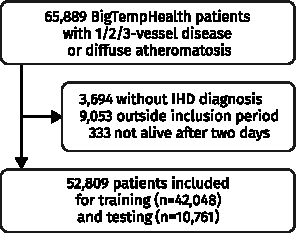
\includegraphics{graphics/pmhnet-v2-inclusion-flowchart.pdf}
    \caption[Inclusion diagram for \pmhnet{2}]{%
        Flow diagram showing the inclusion and exclusion criteria 
        for derivation of thè \pmhnet{2} cohort. An \acs{IHD} diagnosis
        was defined as any prior or concurrent hospital admission with 
        a primary or secondary diagnosis code (\acs{ICD-10}) of I20-25.
        The inclusion period ranged from 01.01.2006 to 31.12.2016, 
        both dates inclusive.}
    \label{fig:pmhnet-v2-inclusion}
\end{marginfigure}
% ←

To test the utility of the presented competing risk methodology,
we set out to develop \pmhnet{2}, a collection of four different 
neural network-based time-to-event prediction models for cause-specific 
post-angiography prognostication in \ac{IHD}.

\subsection{Defining the Derivation Cohort}

For development of the neural network models, 
we linked the \ac{BTH} dataset to 
the \ac{LPR} and the \ac{EDHR}.
From these, 
we identified patients who underwent a \ac{CAG} which led to a diagnosis of
one-, two-, or three-vessel disease or diffuse atheromatosis between January 1,
2006, and December 31, 2016.
Patients were excluded if they lacked an
\acsu{ICD-10} code for \ac{IHD} (I20-25),
were under 18 years at the time of the \ac{CAG},
or did not survive at least two days after the index procedure
(\cref{fig:pmhnet-v2-inclusion}).

\begin{marginfigure}[0em]% →
    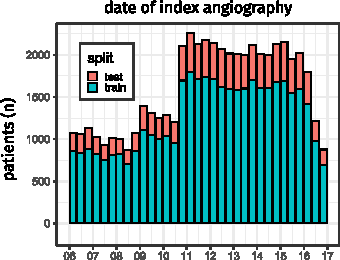
\includegraphics[trim=5mm 0 0 0]{graphics/pmhnet-v2-inclusion-histogram.pdf}
    \caption[Distribution of \pmhnet{2} inclusion times]{%
    Histogram showing the temporal distribution of the \pmhnet{2} index
    coronary angiography procedures. 
    The bars represent the number of patients with an index event in each
    four-month period from 2006 to 2017,
    further segmented to display the proportions of train and test patients.}
    \label{fig:pmhnet-v2-histo}
\end{marginfigure}
% ←

This cohort consists of \num{52809} adults with \ac{IHD}, 
closely resembling and considerably overlapping  
the one used in the \pmhnet{1} study (\studyii{}).
However, unlike \pmhnet{1}, 
which only included 
patients undergoing their first \ac{CAG} 
during the inclusion period,
this study expanded the criteria to 
also include patients with a history of one or more \acp{CAG}.
This approach likely provides 
a more comprehensive representation 
of the diverse manifestations of chronic coronary syndromes.

Prior to statistical analysis and  model training, 
each patient in the development cohort was randomly allocated to the 
training or test split with probabilities of 
\qty{80}{\percent} and \qty{20}{\percent}, 
respectively.
This process resulted in 
a training set of \num{42048} patients 
and a test set of \num{10761} patients
(\cref{fig:pmhnet-v2-histo}).

Serving as model predictors,, 
we identified and created more than 2200 different
features belonging to five different overall categories.
We included 80 clinical features, 418 procedure and examination codes,
785 distinct medical prescriptions, 504 different diagnoses, 
and 475 unique laboratory test features.
Further details on features and the pre-processing 
is included in the manuscript in \cref{chap:study3-paper}.

\subsection{Included Time-to-Event Endpoints}

As the index date, we used the date of the inclusion \ac{CAG}.
For the \pmhnet{2} time-to-event prediction models, 
follow-up was defined as the number of days 
between the index date and the onset of endpoints or censoring,
whichever came first, 
with a maximum follow-up duration of five years.
We defined four different primary outcomes, 
three of which included competing risks:

\begin{marginfigure}[2em]% →
    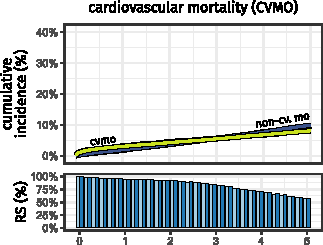
\includegraphics[trim=5mm 0 0 0]{graphics/pmhnet-v2-cvmo-cic.pdf}
    \caption[Cumulative incidence of the \acsfont{CVMO} outcome]{%
        Cause-specific cumulative incidence functions for the 
        \acsfont{CVMO} outcome (cvmo) and the competing endpoint 
        \enquote{non-cardiovascular} mortality. (non-cv. mo). 
        The bottom panels shows the proportion of train/test patients
        still at risk (i.e. non-censored and still alive) 
        at each two-month period following the index \acs{CAG}.}
    \label{fig:pmhnet-v2-cic}
\end{marginfigure}
% ←

\begin{description}
    \item[\acsfont{ACMO}---all-cause mortality,]
        was obtained from the \ac{CPR}
        using the same definition as in \studyii{}.
        \acsfont{ACMO} did not have competing risks.

    \item[\acsfont{CVMO}---cardiovascular mortality,]
        was defined from the \ac{DAR} as deaths where the underlying
        cause of death was assigned an \ac{ICD-10} code from the 
        cardiovascular chapter (I00--99).
        Deaths attributed to different causes  were 
        treated as competing risks, as depicted in \cref{fig:pmhnet-v2-cic}

    \item[\acsfont{CVCO}---cardiovascular complications,] 
        was defined from the \ac{LPR} as a composite outcome 
        covering hospital admissions with a primary diagnosis of
        \enquote{heart failure} (\acs{ICD-10}: I50),
        \enquote{atrial fibrillation or flutter} (I48),
        \enquote{cardiac arrest} (I46),
        and 
        \enquote{cerebrovascular accident} (I61, I63--64)
        and in-hospital procedures for 
        \enquote{implanation of pacemaker} (\acs{SKS}: \texttt{"BFCA0*"})
        and
        \enquote{implanation of cardioverter-defibrillator} (\texttt{"BFCB0*"}).
        Events within four weeks after the index angiography was assumed
        to be unrelated to disease progression and was ignored.
        \acsfont{ACMO} was treated as a competing risk.

    \item[\acsfont{MIEV}---new myocardial ischemia,] 
        was defined from the \ac{LPR} as 
        unplanned \acp{PCI}, \acp{CABG}, or 
        in-hospital admissions longer than \qty{24}{\hour}
        with a primary diagnosis of \ac{IHD} (I20-25).
        Events within the eight weeks after the index \ac{CAG} 
        were not considered \enquote{new} events 
        and were therefore excluded.
\end{description}

\subsection{Neural Network Architecture}

For the \pmhnet{2} models, 
we used a \enquote{ResNet}-inspired neural network architecture
adapted for tabular data, as advocated by \textcite{gorishniyRevisiting2023}.
This architecture consists of multiple so-called residual blocks,
or \enquote{ResBlocks}, sequentially connected to one another.
For \pmhnet{2}, these ResBlocks were defined as
%
\begin{equation}
    \mathrm{ResBlock}_{h}(z) = ( 
    \mathrm{BN} 
    \circ \mathrm{FC}_{h,h} 
    \circ \mathrm{DO} 
    \circ \mathrm{SiLU} 
    \circ \mathrm{FC}_{h,h} 
    \circ \mathrm{DO} 
    )(z)  + z
\label{eq:resblock}%
\end{equation}%
where \(\mathrm{BN}\) is a batch normalization function,
\(\mathrm{FC}_{h,h}\) is a fully-connected linear function
with \(h\) inputs and \(h\) outputs, 
\(\mathrm{DO}\) is a dropout function for regularization,
and \(\mathrm{SiLU}\) is the sigmoid-weighted linear unit (\acsfont{SiLU})%
---a non-linear activation function.
~\autocite{elfwingSigmoidWeighted2017}
An important aspect of the ResBlock is the skip-connection,
\(f(z) + z\), where a learned representation is added on top of 
the untransformed input, which can enable training of
very deep neural networks.
~\autocite{orhanSkip2018}
For the models tested, we constrained all ResBlocks to have the same
number of hidden units \(h\) in each of the hidden layers.

By stacking together several of these building blocks,
we can adjust the depth and complexity of the final architecture
\begin{equation}
    \mathrm{ResNet}(z) = 
    (
    \mathrm{FC}_{m,h} 
    \circ 
    \mathrm{ResBlock}_{h} 
    \circ \dots 
    \circ \mathrm{ResBlock}_{h} 
    \circ \mathrm{FC}_{h,o} 
    )(z)
\end{equation}
which depends on the number of input features \(m\),
the number of hidden units \(m\), 
and the number of output logits \(o\).%
\sidenote{%
    Which for our discrete-time competing risk setup is 
    \(q \cdot (\kappa + 1)\), where \(q\) is the number of time bins
    and \(\kappa\) is the number of competing risks.
}

\section{Model Training and Hyperparameter Tuning}

For training neural network models, 
we utilized the \enquote{super-convergence} training protocol
described by \textcite{smithSuperConvergence2018a},
a general methodology for fast and efficient training of
neural network models.
In this approach, 
models are trained for a pre-specified number of steps
using the \enquote{AdamW} stochastic optimization algorithm,
~\autocite{loshchilovDecoupled2019}
and the learning-rate is continuously adjusted during training
following a one-cycle learning rate policy.
We used the \texttt{OneCycleLR} implementation 
from the \texttt{PyTorch} library.%
\sidecite[0em]{paszkePyTorch2019}

Given the multitude of settings that needs to be specfied
for configuration of both the neural network models and
the training process itself, 
we conducted several \ac{HPO} experiments to
explore various combinations of hyperparameters.
For this purpose, we further subdivided the training data
into a training and validation split.
This validation split was used to assess model performance
of the models constructed during the hyperparameters sweeps.
The following gives an overview of the hyperparameters
included in the \ac{HPO}, and the range of possible values explored.

\begin{fullwidth}
\begin{multicols}{3}
\raggedcolumns

We included five parameters to adjust the architecture of the networks
and the complexity of the discretization grid:
\begin{enumerate}[label=\alph*)]
    \item \verb|n_timebins|:
        number of time bins in the discretization grid.
        Allowed values are 
        \numrange{1}{100}.
    \item \verb|n_hidden|:
        number of hidden units in each hidden layer.
        Controls the width of the neural network.
        Allowed values are 
        \numrange{10}{100}.
    \item \verb|n_blocks|:
        number of residual blocks.
        Controls the depth of the neural network.
        Allowed values are 
        \numrange{1}{20}.
    \item \verb|enable_skipconn|:
        should the skip-connection part of the ResBlock
        (\cref{eq:resblock}) be included? 
        Toggle between true/false.
    \item \verb|enable_batchnorm|:
        should the batch-normalization layer of the ResBlock
        (\cref{eq:resblock}) be included? 
        Toggle between true/false.
\end{enumerate}

Four parameters were used to configure the model training process
and to regulate the amount and type of regularization.
\begin{enumerate}[label=\alph*), resume]
    \item \verb|n_step|:
        number of training epochs.
        Range: \numrange{5}{25}.
    \item \verb|max_lr|:
        maximum learning rate in the one-cycle scheduler.
        Range: \numrange{1e-3}{1}.
    \item \verb|weight_decay|:
        amount of  weight decay used in the \verb|AdamW| optimizer.
        Range: \numrange{1e-5}{1}.
    \item \verb|dropout|:  
        dropout rate. 
        Range: \qtyrange{0}{90}{\percent}.
\end{enumerate}

Finally, four parameters controlled the upper limit on the inclusion of 
retrospective data for various features categories, namely:
\begin{enumerate}[label=\alph*), resume]
    \item \verb|cutoff_bioc|: 
        inclusion window for
        laboratory tests results.
        Range: \numrange{0.5}{5},
        stepsize: \num{0.5} .
    \item \verb|cutoff_diag|:
        inclusion window for
        diagnosis codes.
        Range: \numrange{0.5}{10},
        stepsize:  \num{0.5} .
    \item \verb|cutoff_proc|:
        inclusion window for
        procedure and examination codes.
        Range: \numrange{0.5}{10},
        stepsize: \num{0.5} .
    \item \verb|cutoff_medi|:
        inclusion window for
        drug prescription features.
        Range: \numrange{0.5}{10},
        stepsize: \num{0.5} .
\end{enumerate}
    
\end{multicols}
\end{fullwidth}

The \ac{HPO} process was automatized using the \verb|Optuna| framework.
~\autocite{akibaOptuna2019}
As the tuning parameter,
we used the \ac{IPA} of the primary outcome 
(\acsfont{ACMO}, \acsfont{CVMO}, \acsfont{CVCO}, and \acsfont{MIEV}).
Since the \ac{IPA} is a time-dependent measure,
we calculated the \ac{IPA} at 50 evenly spaced timepoints from
\numrange{0.5}{5} years and numerically integrated the values
to provide a single performance measure for the \ac{HPO}. 

After \ac{HPO}, 
we used the best performing configuration for each outcome
and trained the final models on the entire training data.

\subsection{Model Evaluation}

For evaluation of the \pmhnet{2} time-to-event prediction models,
we assessed model discrimination and calibration. 
Similar to \studyii{}, we used \ac{tdAUC} to quantify the models'
cause-specific ability to discriminate between cases and non-cases.
For quantification of model calibration,
we computed the Brier score and the \ac{IPA}. 

The \ac{IPA},
which is an \(R^{2}\)-type measure of model accuracy,
is obtained by scaling the Brier score 
of the model with that of a covariate-less null model 
based on the estimated incidences from the Kaplan-Meier or Aalen-Johansen
estimator.
~\autocite{kattanIndex2018}
It is sometimes referred to as the \enquote{scaled Brier score}.
One advantage of the \ac{IPA} metric is its easy interpretation:
a perfect model has a score of \qty{100}{\percent},
models with a positive \ac{IPA} are potentially useful,
and models with a negative \ac{IPA} are useless or harmful.

For the three outcomes including competing risks---%
\acsfont{CVMO}, \acsfont{CVCO}, and \acsfont{MIEV}---%
we also included a version of the model where 
competing events were treated as censored.
To analyse the difference between the models 
with and without competing risks, 
we compared the differences in Brier score and \ac{tdAUC}.
Standard errors for the \(\Delta\mathrm{Brier}\) scores are obtained
using an approach similar to that of one-sample t-tests, 
as described in \textcite{gerdsMedical2021}.
Correspondingly, 
standard errors for the \(\Delta \mathrm{AUC}\) 
were obtained using the Delong-Delong method,
~\autocite{delongComparing1988}
also following \textcite{gerdsMedical2021}.

For these model evaluation metrics and tests, 
we use the implementations provided by the R-package \texttt{riskRegression}.
~\autocite{gerdsRiskRegression2023}
All performance metrics were exclusively calculated using 
the test set, or in the case of \ac{HPO}, a validation split of 
the training data.

\section{Main Findings}

We developed neural network models for
time and cause-specific probabilistic predictions of 
experiencing each of the four primary endpoints 
\acsfont{ACMO}, \acsfont{CVMO}, \acsfont{CVCO}, and \acsfont{MIEV}.
From the \ac{HPO} experiments performed on each of these models,
we found that several hyperparameter configurations were associated
with a negative validation-set \ac{IPA} and therefore resulted in 
decidedly inaccurate time-to-event models.
On the other end of the spectrum, 
the best performing configurations for each of the four outcomes
were all found to have useful \ac{IPA} scores,
with 
\qty{22.2}{\percent} for \acsfont{ACMO},
\qty{12.6}{\percent} for \acsfont{CVMO},
\qty{23.5}{\percent} for \acsfont{CVCO},
and 
\qty{8.00}{\percent} for \acsfont{MIEV},
highlighting the importance of the \ac{HPO} process.

From analysis of the \ac{HPO} sweeps,
we found that \verb|enable_batchnorm| and \verb|enable_skipconn| 
considerably affected model accuracy. 
In every case tested, 
we concluded that both parameters should be set to
\verb|true| for optimal performance. 
For trials without skip-connections and batch-normalization,
the model architecture resembles an \ac{MLP}
rather than a ResNet-like one,
which negatively affected model performance.
\textcite{gorishniyRevisiting2023} 
found that a ResNet-like architecture are well-suited for
tabular data neural networks, 
consistently outperforming \ac{MLP}-based models.
Our experiments support this and extend the finding 
to Logistic-Hazard time-to-event models,
both with and without competing risks.


The best-performing configurations, 
as determined by the \ac{HPO} process,
were then used in the setup and training of 
the final \pmhnet{2} models.
These models were then evaluated on 
the previously unseen hold-out test data.
\Cref{fig:pmhnet-v2-calibration,%
      fig:pmhnet-v2-performance,%
      fig:pmhnet-v2-discrimination}
here summarise the main evaluation results,
but additional details are included in
the full-length manuscript in \cref{chap:study3-paper}.

Importantly, models based on our competing risk Logistic-Hazard framework  
were all found to be well-calibrated,
as exemplified by the calibration plots 
in \cref{fig:pmhnet-v2-calibration}.
These plots compare the 1- and 5-year predictions 
with the observed incidences obtained from the Kaplan-Meier
and Aalen-Johansen estimates.

\begin{marginfigure}% →
    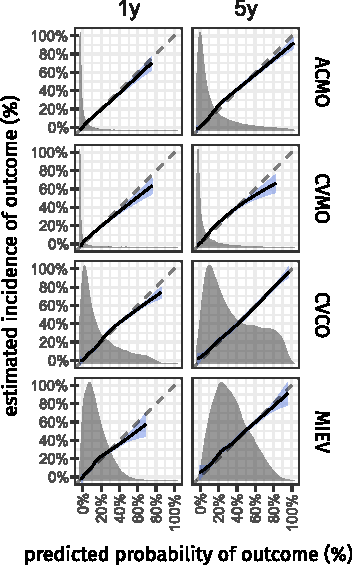
\includegraphics{graphics/pmhnet-v2-visual-calibration.pdf}
    \caption[Calibration of \pmhnet{2} models at 1 and 5 years]{%
        Calibration plots comparing 
        the cause-specific \(t\)-year \pmhnet{2} model predictions 
        with the estimated incidences at a 1 and 5 year prediction horizon.
        The included  regression line is obtained by fitting a natural
        cubic spline (\(d.o.f. = 6\)) with pseudo-values obtained
        by jackknife resampling of the Kaplan-Meier 
        (\acsfont{ACMO})
        or the Aalen-Johansen 
        (\acsfont{CVMO}, \acsfont{CVCO}, and \acsfont{MIEV})
        estimates.
        The dashed 45-degree reference lines represent perfect calibration. 
        The density curve in the background of each panel shows the 
        distribution of the model estimates.
    }
    \label{fig:pmhnet-v2-calibration}
\end{marginfigure}% ←

From visual inspection of the distribution of model predictions 
conditional on the observed outcomes (\cref{fig:pmhnet-v2-discrimination}),
we found the predicted cause-specific probabilities to be consistently higher 
for patients that experience the primary outcome (\enquote{primary})
compared to those that remained event-free (\enquote{event-free}).
This effect, however,  was less pronounced for the \acsfont{MIEV} 
outcome.
Interestingly, for the three outcomes with competing risks;
\acsfont{CVMO}, \acsfont{CVCO}, and \acsfont{MIEV};
the distribution of the primary-cause predictions
between patients experiencing the primary outcome (\enquote{primary})
and those experiencing the competing event (\enquote{competing}),
were overlapping considerably.
This suggests that it is difficult to distinguish between 
the competing risks, perhaps due to many shared risk factors,
indicating that treating competing events as censoring
would invalidate the assumption of uninformative censoring.

\begin{figure}[tpb]% →
    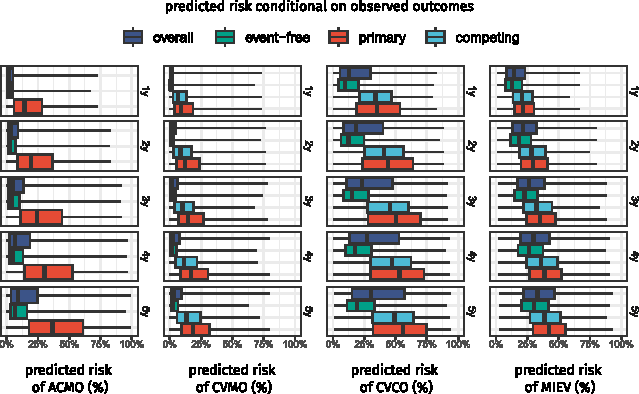
\includegraphics{graphics/pmhnet-v2-visual-discrimination.pdf}
    \caption[Test-set discrimination of \pmhnet{2}]{%
        Visual assessment of test set discrimination.  
        Boxplots display 
        the predicted \(t\)-year risk quantiles for the primary endpoints, 
        conditional on the observed \(t\)-year outcomes observed.  
        The boxplot marked \enquote{overall} show the observed 
        quantiles of the entire test set. 
        The quantiles included in the boxplots marked
        \enquote{primary}, \enquote{competing}, and \enquote{event-free}
        have been estimated using inverse probability of censoring weighting.
     }
    \label{fig:pmhnet-v2-discrimination}
\end{figure}% ←

To further quantify the model discrimination and calibration, 
we calculacted the \ac{tdAUC} and \ac{IPA} across 100 evenly separated
prediction horizons, ranging from 31 days to 5 years 
(\cref{fig:pmhnet-v2-performance}).
From this, we observed good model performance across
all tested prediction horizons.
For the three outcomes including competing risks,
we also included a naïve reference model where 
competing events were treated as censored.
We consistently found the \ac{tdAUC} and \ac{IPA}
of the naïve models to be worse than the competing-risk version.

\begin{figure}% →
    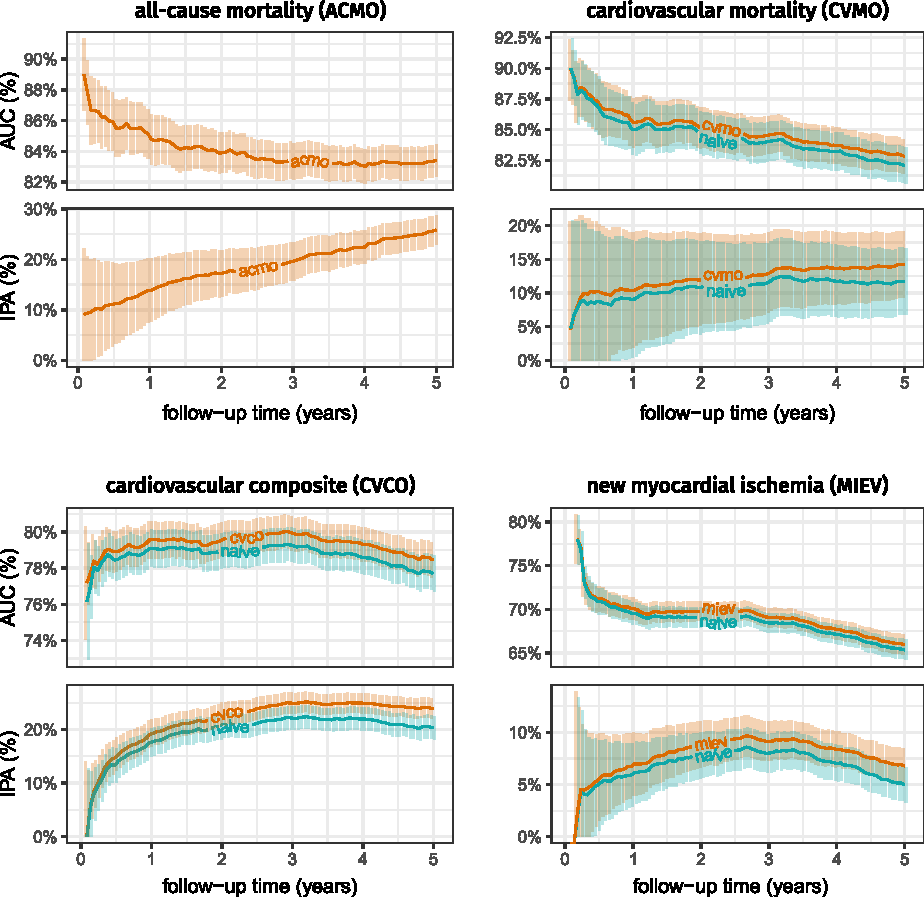
\includegraphics{graphics/pmhnet-v2-metrics.pdf}
    \caption[Test-set performance of \pmhnet{2}][-2em]{%
        \Acf{tdAUC} and \acf{IPA} for prediction of the primary
        endpoint for each of the four \pmhnet{2} models.
        \ac{tdAUC} and \ac{IPA} are computed at 100 evenly spaced
        timepoints, ranging from 31 days to 5 years.
        For the three outcomes including competing risks---%
        \acsfont{CVMO}, \acsfont{CVCO}, and \acsfont{MIEV}---%
        we also included a naïve single-risk model where 
        competing events were treated as censored.%
    }
    \label{fig:pmhnet-v2-performance}
\end{figure}% ←

To test the performance gain of jointly modelling the competing
risks, we analysed the differences in \ac{tdAUC} and Brier scores
between the competing-risk and the naïve versions across
the \acsfont{CVMO}, \acsfont{CVCO}, and \acsfont{MIEV} outcomes.
The results of these comparisons are summarised in \cref{tab:pmhnet-v2-delta},
which shows that in all cases, 
the competing risk models are better or 
comparable to models disregarding competing events.
Specifically, model calibration were found to be the most impacted
performance metric.

\begin{table}% →
    \small
\begin{tabularx}{\linewidth}{Xcccccc}\toprule
     & \multicolumn{3}{c}{ \(\Delta \mathrm{AUC}\)}
     & \multicolumn{3}{c}{ \(\Delta \mathrm{Brier}\)}\\
     \cmidrule(lr){2-4} \cmidrule(lr){5-7}

     & \multicolumn{2}{c}{ \(p < 0.05\)} & \(p \geq 0.05\)
     & \multicolumn{2}{c}{ \(p < 0.05\)} & \(p \geq 0.05\) \\
     \cmidrule(lr){2-3} \cmidrule(lr){4-4}
     \cmidrule(lr){5-6} \cmidrule(lr){7-7} 

     & \(\Delta > 0\) & \(\Delta < 0\) & \(\Delta \approx 0\) 
     & \(\Delta > 0\) & \(\Delta < 0\) & \(\Delta \approx 0\) \\
     \midrule

    \acsfont{CVMO} vs. naïve & 56 & 0 & 44 & 97 & 0 & 3 \\
    \acsfont{CVCO} vs. naïve & 91 & 0 & 9  & 97 & 0 & 3 \\
    \acsfont{MIEV} vs. naïve & 87 & 0 & 13 & 99 & 0 & 1 \\
    \bottomrule
\end{tabularx}
\caption[\pmhnet{2} performance gain by inclusion of competing risks]{%
    Differences in Brier score and \ac{tdAUC} 
    between the \pmhnet{2} competing risk models 
    and naïve reference models were competing events were treated as
    censoring. 
    The table shows the number of timepoints for which 
    the competing risk model had significantly better (\(\Delta > 0\)),
    significantly worse (\(\Delta < 0\)), 
    or comparable performance (\(\Delta \approx 0\))
    to the naïve model. }
\label{tab:pmhnet-v2-delta}
\end{table}% ←

\section{Conclusions}

In this study, we presented the development of \pmhnet{2}, 
an ensemble of four distinct neural network models for time-to-event 
prediction of important clinical outcomes in patients with \ac{IHD}.
These models were developed to predict the onset of important clinical
endpoints following coronary angiography:
all-cause mortality (\acsfont{ACMO}), 
cardiovascular mortality (\acsfont{CVMO}), 
cardiovascular complications (\acsfont{CVCO}), 
and new myocardial ischemia events (\acsfont{MIEV}). 

To enable the construction of these models, 
a central contribution of our research, 
is the development of a novel approach for
neural network-based modelling of 
discrete time-to-event data with competing risks.
This approach can be viewed as an extension to
Logistic-Hazard model from 
\textcite{gensheimerScalable2019},
and is grounded in classical statistical analysis of 
discrete time-to-event data.
~\autocite{tutzModeling2016}
To the best of our knowledge, 
we are the first to utilize this methodology
for neural network-based competing risk analysis.

Our approach has been implemented in the python package \texttt{DiscoTime},
a general-purpose software library that facilitates the application 
and further exploration of this methodology for 
time-to-event prediction with neural networks.
~\autocite{holmDiscotime}

In our experiments, \pmhnet{2} models,
utilizing this novel approach, 
provided accurate and well-calibrated time- and cause-specific 
estimates for secondary prognostication in patients with \ac{IHD}.
Compared to the common practice of treating competing events as censored,
our methodology demonstrated an increase in both model
discrimination and, particularly, in model calibration.
In the context of clinical research where competing risks are common,
this finding underscores the importance of using methodologies, 
like ours, that properly handle competing risks. 
Our study suggests such approaches should be considered in 
the development of future neural network-based medical risk prediction models.
